\newcommand{\sn}[2]{\ensuremath{{#1}\times 10^{#2}}}

\chapter{Imprecise Prior}

When estimating the probabilities for our classifier we take in to account our prior beliefs for them and the likelihood given a set of observations.

When we initially chose our prior distribution we chose the hyperparameters in \cref{initial prior} such that they follow the principal of indifference.
However as previously mentioned this prior does not truly represent a lack of prior knowledge.
We need a way to represent this lack of knowledge and acknowledge that our estimates for the probabilities depend on our choice prior distribution.

\section{Imprecise Dirichlet Model}

The imprecise Dirichlet model is a model for this lack of knowledge introduced by Walley \cite{Walley96}.
Instead of using a single prior distribution to represent our beliefs about the unknown parameters we use a set of prior distributions.

Suppose our objects had no attributes but we are still interested in classifying the object.
In the imprecise Dirichlet models the prior distributions are Dirichlet distributions with parameters $(s, \mathbf{t})$ such that $\sum_{c \in \mathcal{C}} t(c) = 1$.
The distributions for the likelihood are multinomial so:
\begin{equation}
	f(\mathbf{n} \mid \mathbf{\theta}) \propto \prod_{c \in \mathcal{C}} \theta_c^{n(c)}
	\qquad
	f(\mathbf{\theta} \mid s, \mathbf{t}) \propto \prod_{c \in \mathcal{C}} \theta_c^{st(c) - 1}
\end{equation}
Then the posterior distribution is of the form:
\begin{equation} \label{dirichlet_pdf}
	f(\mathbf{\theta} \mid \mathbf{n}, s, \mathbf{t}) \propto \prod_{c \in \mathcal{C}} \theta_c^{n(c) + st(c) - 1}
\end{equation}
which is also a Dirichlet distribution with parameters $(N+s, \frac{\mathbf{n}+s\mathbf{t}}{N+s})$.
We can then take the posterior expectation for the theta chances giving:
\begin{equation}
	P_t(c) = E(\theta_c \mid \mathbf{n}, s, \mathbf{t}) = \frac{n(c)+st(c)}{N+s}
\end{equation}
Note this is a function of $t(c)$ which allow us to obtain upper and lower estimates for for probabilities by varying $t(c)$:
\begin{align}
	\overline{P}(c) & = \frac{n(c)+s}{N+s} & (t(c) \rightarrow 1) \\
	\underline{P}(c) & = \frac{n(c)}{N+s}  & (t(c) \rightarrow 0)
\end{align}

Zaffalon applied this method of imprecise priors to the problem of classification.
We will use a set of the prior distributions of the form in \cref{prior} for a fixed value of $s$.
The parameter $s$ represents the strength of our prior beliefs and determines how quickly our classifier learns.

\section{Imprecise Probabilities}

Imprecise probabilities is a general term for all models which do not assign definite numerical probabilities to events \cite{Walley91}.
Imprecise probabilities have other applications in artificial intelligence and can better represent an experts knowledge \cite{}.
One such approach is to use upper and lower bounds for a probability.
Using the model of imprecise priors we can find the upper and lower bounds for each posterior expectation based on different prior distributions.

Recall that we estimate the probabilities by taking the expectation of the posterior distribution and that these estimates depend on $\mathbf{t}$ i.e.:
\begin{align}
	P_t(c) & = E(\theta_c \mid \mathbf{n},s,\mathbf{t}) = \frac{n(c) + st(c)}{N + s} \\
	P_t(a_i \mid c) & = E(\theta_{a_i \mid c} \mid \mathbf{n},s,\mathbf{t}) = \frac{n(a_i, c) + st(a_i, c)}{n(c) + st(c)}
\end{align}
We can then use these to find upper and lower estimates for the probabilities over all values of $\mathbf{t}$ in our prior model.
For our distributions the upper and lower bounds are given by:
\begin{align}
	\overline{P}(c) & = \frac{n(c) + s}{N+s} \\
	\underline{P}(c) & = \frac{n(c)}{N+s}
\end{align}
These occur when we use the prior distributions with $t(c) \rightarrow 0$ and $t(c) \rightarrow 1$ respectively.

Similarly we have:
\begin{align}
	\overline{P}(a_i \mid c) & = \frac{n(a_i, c) + s}{n(c)+s} \\
	\underline{P}(a_i \mid c) & = \frac{n(a_i, c)}{n(c)+s}
\end{align}
These occur when we use the prior distributions with $t(c) \rightarrow 1$, $t(a_i, c)\rightarrow1$ and $t(c) \rightarrow 1$, $t(a_i, c)\rightarrow0$ respectively.

Let's start by comparing how our classifier behaves if we assume the true probability is at each end of the interval.
We will use the 0-1 loss function for the decision method and estimate each probability $P(\cdot)$ by either the upper or lower probability of our interval.
We will measure accuracy and indeterminate classifications as before.

\begin{center}
	\begin{tabular}{l|c c}
	                & Accuracy & Indeterminate Assignments \\
	\hline
	Lower Estimates & 62.17\%  & 20.02\%            \\
	Upper Estimates & 40.09\%  & 0\%                \\
	\end{tabular}
\end{center}

Neither of these offer a sufficient classification.
There are often no observations of an attribute with a particular class which is why the lower estimates returns indeterminate classifications despite a reasonable accuracy for this data set.
On the other hand when using the upper estimates our classifier has a terrible accuracy.

\section{Simple Credal Classifier}
Alternatively we can turn our classifier into a credal classifier.
A credal classifier assigns a set of classes as opposed to a single class to an object.

Recall the MAP estimate for the risk rating of a vehicle given by \cref{map}.
We say that a class $c'$ is dominated by $c''$ if:
\begin{equation}\label{Credal Dominance}
	P_t(c' \mid \mathbf{a}) < P_t(c'' \mid \mathbf{a})
\end{equation}
for all values of $\mathbf{t}$ in our prior model.
This is because the MAP estimate for the class will always choose $c''$ over $c'$ regardless of which prior is used.
Note that this is equivalent to $P_t(c', \mathbf{a}) < P_t(c'', \mathbf{a})$ as $P(\mathbf{a})$ does not depend on $c$.

We can use the bounds for the probabilities we found earlier to create an interval $P(c, \mathbf{a})$ must lie in. 

If we look at the intervals created by the upper and lower estimates we achieve:
\begin{equation}
	P_t(c, \mathbf{a}) \in \left[ \underline{P}(c)\prod_{i=1}^k \underline{P}(a_i \mid c), \overline{P}(c)\prod_{i=1}^k \overline{P}(a_i \mid c) \right]
\end{equation}
for each $c \in \mathcal{C}$.
This is true because:
\begin{equation}
\underline{P}(c)\prod_{i=1}^k \underline{P}(a_i \mid c) \leq \underline{P}(c, \mathbf{a}) \leq P_t(c, \mathbf{a}) \leq \overline{P}(c, \mathbf{a}) \leq \overline{P}(c)\prod_{i=1}^k \overline{P}(a_i \mid c)
\end{equation}
for all choices of $\mathbf{t}$.
We can use the above intervals to create a simple credal classifier.

For an example consider the following intervals:
\begin{center}
	\begin{tabular}{l|c c}
	Risk Rating & Lower Bound & Upper Bound \\
	\hline
	-2          & $0$              & $\sn{3.12}{-9}$  \\
	-1          & $0$              & $\sn{8.91}{-16}$ \\
	0           & $\sn{3.81}{-15}$ & $\sn{2.30}{-13}$ \\
	1           & $\sn{2.19}{-9}$  & $\sn{2.34}{-8}$  \\
	2           & $\sn{1.88}{-13}$ & $\sn{6.22}{-11}$ \\
	3           & $0$              & $\sn{5.82}{-17}$ \\
	\end{tabular}
\end{center}
We can see the classes -1, 0, 2 and 3 are dominated by 1.
However the risk rating of -2 is not dominated by 1 as $\sn{3.12}{-9} > \sn{2.19}{-9}$.
Hence our credal classifier returns the set or risk ratings $\{-2, 1\}$.
Note that in this particular example the true risk rating was 1 so our credal classifer was correct to include it in the set of possible classes.

We now need a way to test this classifier.
We cannot use our previous measure of accuracy as this classifier may not return a single class.
Instead there are a few metrics we can use for our diagnostics \cite{Antonucci11}:
\begin{description}
	\item[Single Accuracy (A\%)] Accuracy of the credal classifier when a single class is returned
	\item[Set Accuracy (B\%)] Percentage of objects for which the true class is in the returned set when the set has size larger than one
	\item[Indeterminate Output Size (C)] Average set size for returned sets containing more than one class
	\item[Determinacy (D\%)] Percentage of objects for which the returned set contains one class
\end{description}

We will vary the choice of the hyper parameter s when measuring these three statistics to see its effect.
\begin{center}
\begin{tabular}{l|c c c c}
        & A\%     & B\%     & C    & D\%     \\
\hline
s = 0.5 & 77.02\% & 87.05\% & 3.71 & 38.34\% \\
s = 1   & 76.92\% & 90.67\% & 3.75 & 20.20\% \\
s = 2   & 75.00\% & 94.30\% & 4.04 & 3.11\% \\
s = 5   & -       & 97.92\% & 5.22 & 0\%   \\
\end{tabular}
\end{center}

We see that the single accuracy of our classifier slightly decreases for the different $s$ parameters.
We also note that this single accuracy is greater than the accuracy of our corrected naive Bayes classifier on the same data set.
However we notice that varying the $s$ parameter has an effect on the other two metrics.
Increasing the value of $s$ decreases determinacy and increases the set accuracy.

This effect can be easily explained.
Increasing the $s$ value increases the upper bound and decreases the lower bound on each of the probabilities being estimated.
Hence increasing the value of $s$ increases the size of the interval and increasing the size of the interval leads to less intervals being dominated and less classes being excluded.

\section{The Naive Credal Classifier}
In the simple credal classifier we estimated the lower and upper bounds for each probability separately using our imprecise prior model.
We then used these separate estimates to make inferences about the true probability of interest: $P(c \mid \mathbf{a})$.

However an alternate method for credal classification was proposed by Zaffalon \cite{Zaffalon01} which we will outline in this section.
This classifier is known as the naive Credal classifier (NCC) and can be more determinate than the simple credal classifier we studied earlier.

Zaffalon has provided multiple examples of this classifier in action.

In one such study he applies the naive Credal classifier to dementia diagnosis \cite{Zaffalon03}.
He starts with a data set containing test results for 3385 different patients split in to five different categories (four describing types of dementia suffers, one describing normal patients).
The data set also contains missing values for some of the patient's test results.
In the first part of the study he simple distinguishes between dementia sufferers and non-dementia sufferers.
In this part the NCC is able to isolate a single class about 90\% of the time and in these cases is accuracy 95\% of the time.
When it fails to isolate a single class the NBC is only able to classify the same object correctly 70\% of the time.
In the second part he limits the study to the type of dementia thus reducing the data set  1103 observations.
Here we see similarly positive results; when the NCC isolates a single class it is accurate 94\% of the time and when it outputs more than one class the set size is about 2 on average and the true class is in this set 98\% of the time.
This study gives an example when a large data set can lead to the NCC being highly determinate and accurate.

In another study he applies the NCC to environmental mining data \cite{Zaffalon02}.
Here the data falls in to one of four categories however the data set only consists of 155 complete instances which is much closer in size to our insurance problem.
In this study the NCC only produced a single class 60\% of the time and of these classes had a single accuracy of 52\%.
When returning more than one class the true class was contained in the output set 82\% of the time.
In comparison the NBC had an accuracy of 48\% on the whole data set and 43\% on the subset of objects the NCC was indeterminate about.
This provides a good example of a situation where the NCC will withhold judgement due to a lack of information.

To define the naive Credal classifier we first rewrite our original definition of credal dominance \cref{Credal Dominance} as:
\begin{equation}
	\frac{P_t(c' \mid \mathbf{a})}{P_t(c'' \mid \mathbf{a})} = \frac{P_t(c')\prod_{i=1}^{k}P_t(a_i \mid c')}{P_t(c'')\prod_{i=1}^{k}P_t(a_i \mid c'')} > 1
\end{equation}
Note that the equality holds because the constant $P(\mathbf{a})$ is cancelled.

If we plug in the posterior expectation for our parametrisation as an estimate for the probabilities then we arrive at:
\begin{equation}
	\frac{n(c')+st(c')}{n(c'')+st(c'')} \prod_{i=1}^k \frac{n(a_i, c') + st(a_i , c')}{n(c'') + st(c'')} \frac{n(c'') + st(c'')}{n(a_i, c') + st(a_i , c')} > 1
\end{equation}

To determine whether this inequality holds we can solve the optimization problem:
\begin{align}
	\min & \left[ \frac{n(c'')+st(c'')}{n(c')+st(c')} \right]^{k-1} \prod_{i=1}^k \frac{n(a_i, c') + st(a_i , c')}{n(a_i, c'') + st(a_i , c'')} \\
	\text{s.t.} & \sum_{c \in \mathcal{C}} t(c) = 1 \\
	& 0 < t(a_i, c) < t(c)
\end{align}
Then compare the answer to 1.
This is the same optimization problem as described by Zaffalon \cite{Zaffalon01}.

It is possible to manipulate this problem into an easier to solve form.
Firstly note that the minimum is achieved when each $t(a_i, c') \rightarrow 0$ and $t(a_i, c'') \rightarrow t(c'')$ so we can use these values in the objective function.
Furthermore, at the minimum, we have $t(c') = 1 - t(c'')$.
To simplify the problem set $st(c'') = x$ then our optimization problem becomes a problem in a single variable:
\begin{align} \label{Credal Dominance Test}
	\min \quad & f(x) = \left[ \frac{n(c'') + x}{n(c') + s - x} \right]^{k-1} \prod_{i=1}^k \frac{n(a_i, c')}{n(a_i, c'') + x} \\
	\text{s.t.} \quad & 0 < x < s
\end{align}

Before we solve this optimization problem we can rule out an edge case.
If $n(a_i, c')=0$ for any $a_i$ then the $c'$ does not dominate $c''$.
IF $n(a_i, c'')=0$ for any $a_i$ then we set $f(0)=10$ to indicate domination is achieved at this point.

Next step is to figure out what the objective function looks like.
Note that it's always positive so if we take the log of $f$ and differentiate we get:
\begin{equation}
	\frac{d\ln(f)}{dx} = \frac{k-1}{n(c'')+x} + \frac{k-1}{n(c')+1-x} - \sum_{i-1}^k \frac{1}{n(a_i, c'') + x}
\end{equation}
Differentiating again gives:
\begin{equation}
	\frac{d^2\ln(f)}{dx^2} = -\frac{k-1}{(n(c'') + x)^2} + \frac{k-1}{(n(c')+1-x)^2} + \sum_{i=1}^k \frac{1}{(n(a_i, c'') + x)^2}
\end{equation}
This is always positive hence the objective function is log concave.
As the logarithm is monotone it follows that $f(x)$ is also concave and hence has a single minimum.

If we remove the edge cases described above we are left with the simple problem of finding the maximum of a concave function in a given interval.
To do so we use the fminbound function in the SciPy library which uses Brent's method \cite{fminbound}.

% If we remove the edge case described above we can compute $f(x)$ for any $x \in [0, s]$.
% There are three cases for finding the minimum:
% \begin{itemize}
% 	\item[$\frac{d\ln f(0)}{dx} \geq 0$] then the minimum is achieved for $x<0$ and hence the minimum in this interval is $f(0)$
% 	\item[$\frac{d\ln f(s)}{dx} \leq 0$] then the minimum is achieved for $x>s$ and hence the minimum in this interval is $f(s)$
% 	\item[Otherwise] the minimum is located within this interval and we can approximate it numerically
% \end{itemize}

\section{Results}

We will measure the same metrics as previously for this new classifier.
The results from 10-fold cross validation with varying $s$ values are as follow:

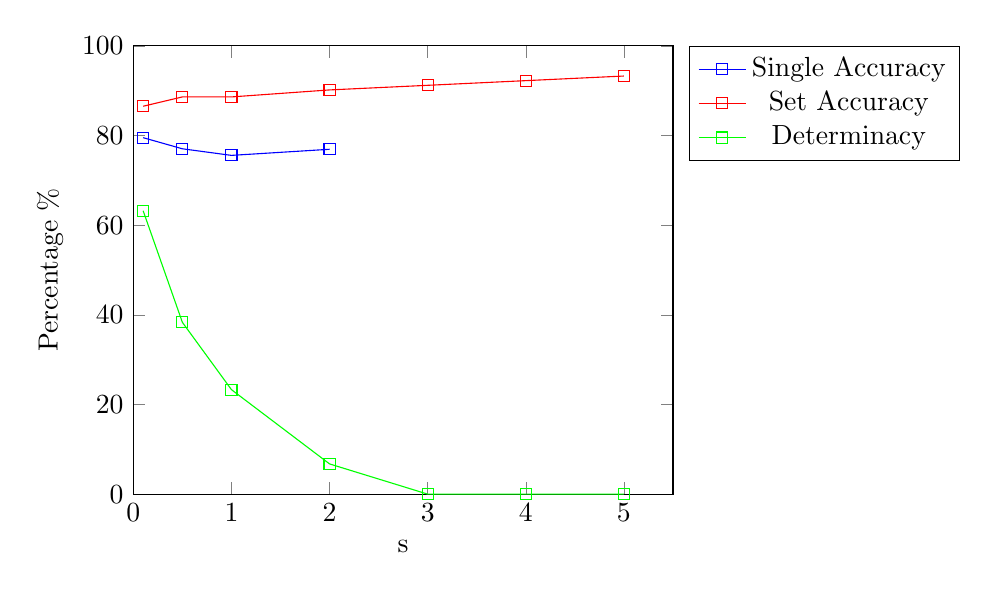
\begin{tikzpicture}
\begin{axis}[
    xlabel={s},
    ylabel={Percentage \%},
    xmin=0, xmax=5.5,
    ymin=0, ymax=100,
	legend pos=outer north east
]

\addplot[
    color=blue,
    mark=square,
    ]
    coordinates {
    (0.1,79.51)(0.5,77.03)(1,75.56)(2,76.92)
    };
    \label{sng_acc}

\addplot[
    color=red,
    mark=square,
    ]
    coordinates {
    (0.1,86.52)(0.5,88.60)(1,88.60)(2,90.16)(3, 91.19)(4, 92.23)(5,93.26)
    };
    \label{set_acc}
 
\addplot[
    color=green,
    mark=square,
    ]
    coordinates {
    (0.1,63.21)(0.5,38.32)(1,23.31)(2,6.74)(3, 0)(4, 0)(5,0)
    };
    \label{det}

\addlegendimage{/pgfplots/refstyle=sng_acc}\addlegendentry{Single Accuracy}
\addlegendimage{/pgfplots/refstyle=set_acc}\addlegendentry{Set Accuracy}
\addlegendimage{/pgfplots/refstyle=det}\addlegendentry{Determinacy}
\end{axis}

\end{tikzpicture}

Additionally we have the following measurements for indeterminate output size:
\begin{center}
\begin{tabular}{c|c c c c}
s & 0.5 & 1 & 2 & 5 \\
\hline
Indeterminate Output Size & 3.65 & 3.66 & 3.74 & 4.25
\end{tabular}
\end{center}

First we note the increase in indeterminate output size and decrease in determinacy.
These are due to the domination criteria becoming harder to satisfy for larger $s$ values.
This leads to less classes being credally dominated and larger output size.

This can also explain the slight trends in single and set accuracy.
Set accuracy increases because the indeterminate output size is always increasing so for each increase in $s$ value we are more likely to see the true class added to the oupur set if it was not already there.
On the other hand the single accuracy does not change much.
As we increase the $s$ value we decrease the number of single outputs and it would appear the outputs that become indeterminate are equally likely to be correct classifications as incorrect classifications.

We can also directly compare the classifications of the naive Credal classifier to those of our interval based classifier. For $s=1$ we have:
\begin{center}
\begin{tabular}{l|c c c c}
         & A\%     & B\%     & C    & D\%     \\
\hline
Interval & 75.61\% & 89.12\% & 3.71 & 21.32\% \\
NCC      & 75.56\% & 88.60\% & 3.66 & 23.31\% \\
\end{tabular}
\end{center}
Here we see similar set and single accuracies.
However we see that the naive Credal classifier is more determinate than the interval based classifier and, when indeterminate, has a smaller average output size.

Our data set only contains observations of three vehicles with risk rating -2.
This means that our credal classifiers struggle to eliminate this classification as an option.
When we consider situations where the NCC is indeterminate and returns two possible classes -2 is always one of these classes.
Additionally the other class is the correct classification 88.60\%.
This is a good example of a situation where the NCC reserves judgement due to lack of observations.